\documentclass[12pt]{article}

\usepackage{amsmath, mathtools}
\usepackage{amsfonts}
\usepackage{amssymb}
\usepackage{graphicx}
\usepackage{colortbl}
\usepackage{xr}
\usepackage{hyperref}
\usepackage{longtable}
\usepackage{xfrac}
\usepackage{tabularx}
\usepackage{appendix,float}
\usepackage{siunitx}
\usepackage{booktabs}
\usepackage{caption}
\usepackage{pdflscape}
\usepackage{afterpage}
\usepackage[none]{hyphenat}
\usepackage[document]{ragged2e}
\usepackage[round]{natbib}

%\usepackage{refcheck}

\hypersetup{
    bookmarks=true,         % show bookmarks bar?
      colorlinks=true,       % false: boxed links; true: colored links
    linkcolor=red,          % color of internal links (change box color with linkbordercolor)
    citecolor=green,        % color of links to bibliography
    filecolor=magenta,      % color of file links
    urlcolor=cyan           % color of external links
}

%% Comments

\usepackage{color}

\newif\ifcomments\commentstrue %displays comments
%\newif\ifcomments\commentsfalse %so that comments do not display

\ifcomments
\newcommand{\authornote}[3]{\textcolor{#1}{[#3 ---#2]}}
\newcommand{\todo}[1]{\textcolor{red}{[TODO: #1]}}
\else
\newcommand{\authornote}[3]{}
\newcommand{\todo}[1]{}
\fi

\newcommand{\wss}[1]{\authornote{blue}{SS}{#1}} 
\newcommand{\plt}[1]{\authornote{magenta}{TPLT}{#1}} %For explanation of the template
\newcommand{\an}[1]{\authornote{cyan}{Author}{#1}}

%% Common Parts

\newcommand{\progname}{Mechatronics} % PUT YOUR PROGRAM NAME HERE
\newcommand{\authname}{Team \#20, Team Name
\\ Robert Zhu zhul49
\\ Zifan Meng mengz17
\\ Jiahui Chen chenj194
\\ Kelvin Huynh huynhk12
\\ Runze Zhu zhur25
\\ Mirza Nafi Hasan hasanm21} % AUTHOR NAMES                  

\usepackage{hyperref}
    \hypersetup{colorlinks=true, linkcolor=blue, citecolor=blue, filecolor=blue,
                urlcolor=blue, unicode=false}
    \urlstyle{same}
                                


% For easy change of table widths
\newcommand{\colZwidth}{1.0\textwidth}
\newcommand{\colAwidth}{0.13\textwidth}
\newcommand{\colBwidth}{0.82\textwidth}
\newcommand{\colCwidth}{0.1\textwidth}
\newcommand{\colDwidth}{0.05\textwidth}
\newcommand{\colEwidth}{0.8\textwidth}
\newcommand{\colFwidth}{0.17\textwidth}
\newcommand{\colGwidth}{0.5\textwidth}
\newcommand{\colHwidth}{0.28\textwidth}

% Used so that cross-references have a meaningful prefix
\newcounter{defnum} %Definition Number
\newcommand{\dthedefnum}{GD\thedefnum}
\newcommand{\dref}[1]{GD\ref{#1}}
\newcounter{datadefnum} %Datadefinition Number
\newcommand{\ddthedatadefnum}{DD\thedatadefnum}
\newcommand{\ddref}[1]{DD\ref{#1}}
\newcounter{theorynum} %Theory Number
\newcommand{\tthetheorynum}{T\thetheorynum}
\newcommand{\tref}[1]{T\ref{#1}}
\newcounter{tablenum} %Table Number
\newcommand{\tbthetablenum}{T\thetablenum}
\newcommand{\tbref}[1]{TB\ref{#1}}
\newcounter{assumpnum} %Assumption Number
\newcommand{\atheassumpnum}{P\theassumpnum}
\newcommand{\aref}[1]{A\ref{#1}}
\newcounter{goalnum} %Goal Number
\newcommand{\gthegoalnum}{P\thegoalnum}
\newcommand{\gsref}[1]{GS\ref{#1}}
\newcounter{instnum} %Instance Number
\newcommand{\itheinstnum}{IM\theinstnum}
\newcommand{\iref}[1]{IM\ref{#1}}
\newcounter{reqnum} %Requirement Number
\newcommand{\rthereqnum}{P\thereqnum}
\newcommand{\rref}[1]{R\ref{#1}}
\newcounter{nfrnum} %NFR Number
\newcommand{\rthenfrnum}{NFR\thenfrnum}
\newcommand{\nfrref}[1]{NFR\ref{#1}}
\newcounter{lcnum} %Likely change number
\newcommand{\lthelcnum}{LC\thelcnum}
\newcommand{\lcref}[1]{LC\ref{#1}}

\usepackage{fullpage}

\newcommand{\deftheory}[9][Not Applicable]
{
\newpage
\noindent \rule{\textwidth}{0.5mm}

\paragraph{RefName: } \textbf{#2} \phantomsection 
\label{#2}

\paragraph{Label:} #3

\noindent \rule{\textwidth}{0.5mm}

\paragraph{Equation:}

#4

\paragraph{Description:}

#5

\paragraph{Notes:}

#6

\paragraph{Source:}

#7

\paragraph{Ref.\ By:}

#8

\paragraph{Preconditions for \hyperref[#2]{#2}:}
\label{#2_precond}

#9

\paragraph{Derivation for \hyperref[#2]{#2}:}
\label{#2_deriv}

#1

\noindent \rule{\textwidth}{0.5mm}

}

\begin{document}

\title{Software Requirements Specification for \progname: ASL Translator} 
\author{\authname}
\date{\today}

\maketitle

~\newpage

\pagenumbering{roman}

\tableofcontents

~\newpage

\section*{Revision History}

\begin{tabularx}{\textwidth}{p{4cm}p{2cm}X}
\toprule {\bf Date  } & {\bf Version} & {\bf Notes}\\
\midrule
October 05, 2022 & 1.0 & Everyone -> Initial SRS Draft\\

\bottomrule
\end{tabularx}

~\newpage

\section{Reference Material}

\subsection{Terms, Abbreviations, and Acronyms}

\renewcommand{\arraystretch}{1.2}
\noindent \begin{tabularx}{\textwidth}{p{0.3\linewidth}|X}
\toprule
\textbf{Term, Abbreviation, or Acronym} & \textbf{Description}\\
\midrule
A
& Shorthand for Assumption\\
\hline
ASL
& Shorthand for American Sign Language. It is a form of sign language primarily used in the US and in parts of Canada\\
\hline
CFR
& Shorthand for Camera Functional Requirement\\
\hline
CMC
& Shorthand for carpometacarpal. This is the joint that connects your thumb to the rest of your hand\\
\hline
DIP
& Shorthand for distal interphalangeal. This is the joint on your finger just before where your fingernail is\\
\hline
IP
& Shorthand for interphalangeal. This is the joint just before where your fingernail on the thumb is situated\\
\hline
PIP 
& Shorthand for proximal interphalangeal. This is the next joint up your finger from where the knuckles are\\
\hline
MCP
& Shorthand for metacarpophalangeal. This is the joint situated roughly where your knuckles are\\
\hline
ML
& Shorthand for Machine Learning\\
\hline
MLFR
& Shorthand for Machine Learning Functional Requirement\\
\hline
NFR
& Shorthand for Non-Functional Requirement\\
\hline
CV
&Shorthand for computer vision, computer vision is an interdisciplinary scientific field that deals with how computers can gain high-level understanding from digital images or videos.\\
\hline
OpenCV
& Shorthand for computer vision, computer vision is an interdisciplinary scientific field that deals with how computers can gain high-level understanding from digital images or videos.\\
\hline
TensorFlow
& An open-source framework developed by Google, which enables machine learning, deep learning, and other 
statistical and predictive analytics\\
\bottomrule
\end{tabularx}

\newpage

\pagenumbering{arabic}

\section{Introduction}
\subsection{Purpose of the Project}
The purpose of our project is to create a device that will translate sign language gestures into their corresponding words or phrases. This will require
the creation and development of a computer vision system alongside a machine learning model that will be used to recognize the hand motions, as well as a 
Raspberry Pi that will speak the word or phrase. The user will perform the sign language motion that will be captured by our computer vision system through
a camera, and processed by our machine learning model and spoken through our Raspberry Pi.\\

\subsection{Scope} 
\subsubsection{In-Scope} \label{sec_inScope}
\indent The goals for our project are listed in the following table. The primary goals for our project include
\begin{itemize}
    \item Accurate hand motion recognition: Tracking and recognition of the user\textquotesingle s hands
    \item Real-time translation: Recognition and translation of user\textquotesingle s hand gestures with minimal delay
\end{itemize}

\renewcommand{\arraystretch}{1.2}
\noindent \begin{tabularx}{\textwidth}{p{0.2\linewidth}|p{0.72\linewidth}}
\toprule
\textbf{Goals} & \textbf{Desciption}\\
\midrule
Reliable and Accurate Translations
& The Sign Language Translator requires extensive training on the sensors to capture precise hand motion
and ignore any human error on the user\textquotesingle s part. The processing unit should be able to identify each letter 
within the American Sign Language using the data collected and transmit dialogue accurately to the user\textquotesingle s 
request.\\
\hline
Real Time Translations
& User\textquotesingle s should never be required to wait an extensive period of time for the device to process their hand 
motion and provide a translation. The Sign Language Translator should simulate a real time conversation between
regular people to deliver a seamless transition for other parties during presentations or social interactions.\\
\hline
Ease of Use
& The user experience is crucial for a communication device. The Sign Language Translator should require minimal 
time and effort to set up. Once set up, the device should not require much maintenance or updates. Most importantly,
the device should not hinder the user\textquotesingle s ability to perform the gestures and hand motions of sign language.\\
\hline
Affordability
& The Sign Language Translator should be affordable for the end users as to reduce the need of requiring an actual 
translator to accompany the user during their tasks. The device should remain functional whenever it is required to 
be used, and the hardware components of the device should be simple and cost-effective.\\
\hline
Customizable to User
& As with language, different people might have a certain way of pronouncing a phrase or word and likewise the same 
could be said with Sign Language with slightly different gestures. The device should be able to adapt to the user and 
recognize the unique motions instead of forcing the user to slow down for the device.\\
\bottomrule
\end{tabularx}

\subsubsection{Out-of-Scope}
\indent The stretch goals for our project are listed in the following table. These goals are out-of-scope for our 
project. They may or may not be achieved depending on our progress and time remaining in the academic year.

\renewcommand{\arraystretch}{1.2}
\noindent \begin{tabularx}{\textwidth}{p{0.2\linewidth}|p{0.72\linewidth}}
\toprule
\textbf{Stretch Goals} & \textbf{Desciption}\\
\midrule
Portable
& The final device, while requiring OpenCV to scan and process hand motion, should become more portable and lightweight 
for the user to move around, so as to not interfere with the user\textquotesingle s regular activities. The translator text to speech 
should become an application on all phone brands as for any user with the required equipment to be able to begin using.\\
\hline
Expanding to Different Languages
& As a universal sign language does not exist at the moment, there exists deaf/mute individuals who use another form of 
sign language other than the American Sign language. These include the British, Australian and New Zealand Sign Language (BANZSL),
the Chinese Sign Language (CSL), Arabic Sign language, and much more. The device should be able to understand and translate these 
new hand motions and generate a translation in their native language for this product to be used on a global scale.\\
\hline
Sign Language Education
& The final device should be able to recognize the different hand motions and gestures of sign language in order to accurately
translate them. This would make the device an excellent educational tool for those looking to learn sign language. The device 
could provide feedback and tell users how to improve their gestures using it\textquotesingle s accurate hand tracking to help teach those unfamiliar 
with sign language.\\
\hline
Non-real Time Translations
& The final product should be able to extract and recognize hand gestures from photos or videos uploaded by the users. 
In this case, if the users find online photos or videos related to sign language, they can upload them to application/software
to acquire text-based translation. This could help the users learn sign language from online sources.\\
\bottomrule
\end{tabularx}

\subsection{Usual Operations}
The ASL translator will translate sign language gestures into their corresponding words or phrases to help the daily communication 
for people who have hearing problems. The camera on the device will actively detect the location and the motion of the hand gestures 
of the users standing in front of the camera. Then the computer vision and machine learning algorithm in the device will accurately 
translate the motion of the hands and output the correct English words or phrases. Then, the speaker on the Raspberry Pi which is connected 
to the translator will “speak out” the words or phrases.\\

\subsection{Users and Stakeholders}
The stakeholders for our project are people who have hearing problems and need to use sign language for their daily communication. This 
can also include various accessibility services for various companies, whether that be in education or entertainment. This can also be 
individuals looking to learn sign language as the device can be used as a practice tool to validate their signing. Our project can benefit 
anyone or anything that requires a sign language interpreter.\\

\section{Project Constraints}
\subsection{Constraints}
The project is constrained by the following:
\begin{itemize}
  \item Translate a subset of the American Sign Language (ASL)
  \begin{itemize}
    \item Training a machine learning model to encompass the entire ASL would be very time-inefficient for the time constraint of the project
  \end{itemize}
    \item The project expenses cannot exceed \$750 CAD
  \begin{itemize}
    \item Additionally the project cannot be an off-the-shelf solution and be cost-efficient to attain our goal of affordability
  \end{itemize}
  \item The project must be completed during the course of the academic year
  \begin{itemize}
    \item This serves as a time constraint for the project and is also a requirement set by the course
  \end{itemize}
  \item The area of detection is limited
  \begin{itemize}
    \item Since there is only a specific field of view that can be detected by the camera, the users have to stand at the specific location 
    to ensure the hand motion can be detected by the camera
  \end{itemize}
\end{itemize}

\subsection{Assumptions}

\renewcommand{\arraystretch}{1.2}
\noindent \begin{tabularx}{\textwidth}{p{0.12\linewidth}|p{0.4\linewidth}|p{0.4\linewidth}}
\toprule
\textbf{Identifier} & \textbf{Assumption} & \textbf{Rationale}\\
\midrule
A1 
& Lighting will be sufficient enough for hand joint detection by camera 
& The CV system will require a camera to detect motion. That camera must be able to see the user clearly, 
which will require adequate lighting conditions\\
\hline
A2
& The user is signing ASL and not any other sign language
& The translator will only be able to recognize ASL and for such reasons will not recognize any other sign language 
which could result in a mistranslation or inaccuracy\\
\hline
A3
& The camera or the device containing the camera is portable
& Since the ASL is invented to help daily activities, the camera that is used to detect the hand motion should be compact and light\\
\bottomrule
\end{tabularx}

\subsection{Undesired Event Handling}
In the case of any undesired event, the device should alert the user of the failure or error 
that occurs. This will be crucial during testing as we will need it to ensure our project functions
the way we would like it to. Some potential undesired events could include.
\begin{itemize}
    \item Camera error
    \item Text-to-Speech failure
    \item Faulty training models
\end{itemize}
More undesired events will be added as development continues


\section{Context Diagrams}

\begin{figure}[H] 
\centering
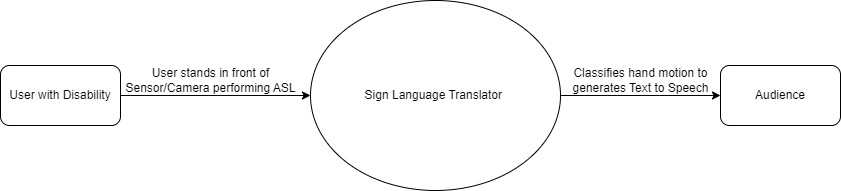
\includegraphics[width=\textwidth,height=0.88\textheight,keepaspectratio]{Context Diagram} 
\caption{Context Diagram} 
\label{Fig.Context_Diagram} 
\end{figure}

\section{Functional Decomposition}
\subsection{Data Flow Model}

\newpage
\subsection{Monitor and Controlled Variables}
\subsubsection{Monitor Variables}

\renewcommand{\arraystretch}{1.2}
\noindent \begin{tabularx}{\textwidth}{p{0.4\linewidth}|p{0.4\linewidth}}
\toprule
\textbf{Variable} & \textbf{Description}\\
\midrule
0. WRIST 
& Wrist \\
\hline
1. THUMB\_JOINT\_0
&CMC joint of the thumb\\
\hline
2. THUMB\_JOINT\_1
&MCP joint of the thumb\\
\hline
3. THUMB\_JOINT\_2
&IP joint of the thumb\\
\hline
4. THUMB\_TIP
&Tip of the thumb\\
\hline
5. INDEX\_JOINT\_0
&MCP joint of the index finger\\
\hline
6. INDEX\_JOINT\_1
&PIP joint of the index finger\\
\hline
7. INDEX\_JOINT\_2
&DIP joint of the index finger\\
\hline
8. INDEX\_JOINT\_TIP
&Tip of the index finger\\
\hline
9. MIDDLE\_JOINT\_0
&MCP joint of the middle finger\\
\hline
10. MIDDLE\_JOINT\_1
&PIP joint of the middle finger\\
\hline
11. MIDDLE\_JOINT\_2
&DIP joint of the middle finger\\
\hline
12. MIDDLE\_JOINT\_TIP
&Tip of the middle finger\\
\hline
13. RING\_JOINT\_0
&MCP joint of the ring finger\\
\hline
14. RING\_JOINT\_1
&PIP joint of the ring finger\\
\hline
15. RING\_JOINT\_2
&DIP joint of the ring finger\\
\hline
16. RING\_JOINT\_TIP
&Tip of the ring finger\\
\hline
17. LITTLE\_JOINT\_0
&MCP joint of the little finger\\
\hline
18. LITTLE\_JOINT\_1
&PIP joint of the little finger\\
\hline
19. LITTLE\_JOINT\_2
&DIP joint of the little finger\\
\hline
20. LITTLE\_JOINT\_TIP
&Tip of the little finger\\
\bottomrule
\end{tabularx}
~\\
Variables above are monitor variables for the left hand, monitor variables for the right hand are similar, the only difference is variable names have \_R at the end. For example, CMC joint of the thumb for the right hand is THUMB\_JOINT\_0\_R.

\begin{figure}[H] 
\centering
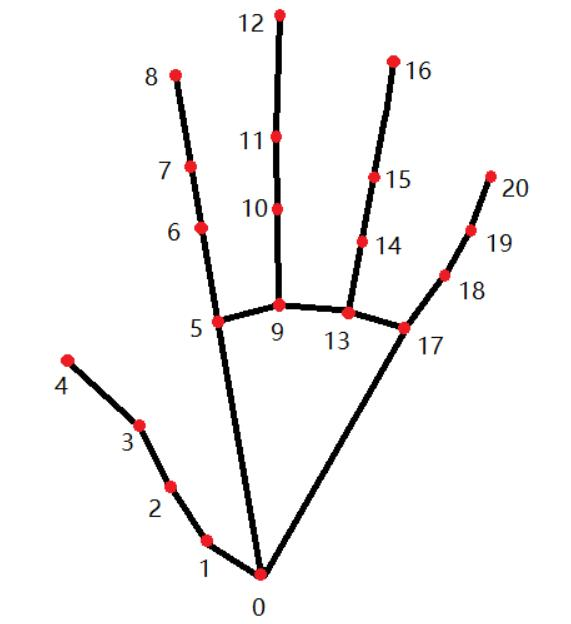
\includegraphics[width=\textwidth,height=0.88\textheight,keepaspectratio]{Hand.jpg} 
\caption{Hand Variables} 
\label{Fig.Monitor_Variables} 
\end{figure}

\subsubsection{Controlled Variables}

\renewcommand{\arraystretch}{1.2}
\noindent \begin{tabularx}{\textwidth}{p{0.4\linewidth}|p{0.4\linewidth}}
\toprule
\textbf{Variable} & \textbf{Description}\\
\midrule
WRIST\_CAL 
& Calibration point for wrist on the camera screen. The x, y, z location of this point must align with the x, y, z location of variable "WRIST" for successful calibration\\
\hline
INDEX\_JOINT\_0\_CAL
& Calibration point for MCP joint of the index finger on the camera screen. The x, y, z location of this point must align with the x, y, z location of variable "INDEX\_JOINT\_0" for successful calibration\\
\hline
LITTLE\_JOINT\_0\_CAL
& Calibration point for MCP joint of the little finger on the camera screen. The x, y, z location of this point must align with the x, y, z location of variable "LITTLE\_JOINT\_0" for successful calibration\\
\bottomrule
\end{tabularx}

\section{Functional Requirements}
\subsection{Camera Functional Requirements}

\renewcommand{\arraystretch}{1.2}
\noindent \begin{tabularx}{\textwidth}{p{0.12\linewidth}|p{0.4\linewidth}|p{0.4\linewidth}}
\toprule
\textbf{Identifier} & \textbf{Requirement} & \textbf{Rationale}\\
\midrule
CFR1 
& User hand gestures should be recognized and converted into input for the system 
& This is the primary and only way that the end user engages with the system. This is to ensure that 
their signing is picked up by the camera within a certain degree of accuracy\\
\hline
CFR2
& The camera must be able to relay its vision back to the program
& This enables validation and testing on the development end. In addition to understanding what needs 
to be corrected to ensure accurate user input\\
\bottomrule
\end{tabularx}

\subsection{Machine Learning Functional Requirements}

\renewcommand{\arraystretch}{1.2}
\noindent \begin{tabularx}{\textwidth}{p{0.12\linewidth}|p{0.4\linewidth}|p{0.4\linewidth}}
\toprule
\textbf{Identifier} & \textbf{Requirement} & \textbf{Rationale}\\
\midrule
MLFR1 
& The program should be able to recognize user hand joints
& This enables the ML model to compare and match user hand gestures to ASL\\
\hline
MLFR2 
& The program should output the x, y, and z coordinates of each joint relative to the camera
& This will enable system calibration and aid in enhancing predictive accuracy as the training 
data set will be primarily static images in contrast to the dynamic input from the end product\\
\hline
MLFR3 
& The program should recognize up to two hands in the input
& The complexity of sign language calls for two hands to enable effective communication. 
Tracking one hand should also be considered as there are words in sign language that require the 
use of a single hand\\
\hline
MLFR4 
& The program should be able to process data in real-time
& The translator should relay the relevant translation within a reasonable amount of time to ensure 
conversation fluidity\\
\hline
MLFR5 
& The program must be able to calibrate the camera
& This is to ensure that the image being processed is undistorted and recognizable to the program 
to prevent inaccuracies and incorrect output from the ML model\\
\hline
MLFR6 
& The program should be calibrated to match the speed of the signer
& The translator should be able to keep up with the user or the likelihood of a mistranslation will increase\\
\hline
MLFR7 
& The ML model should be easily trainable
& This is how the ML model should learn sign language to use in processing. Making it easily trainable should 
enable expandability as well. In addition, this will enable the program to adapt to users\textquotesingle \ specific signing 
habits and allow for manual correction for the future\\
\bottomrule
\end{tabularx}

\section{Functional Requirement Change Likelihood}
\subsection{Camera Functional Requirements}

\renewcommand{\arraystretch}{1.2}
\noindent \begin{tabularx}{\textwidth}{p{0.12\linewidth}|p{0.15\linewidth}|p{0.3\linewidth}|p{0.3\linewidth}}
\toprule
\textbf{Identifier} & \textbf{Likelihood of Change} & \textbf{Rationale} & \textbf{What May Be Changed}\\
\midrule
CFR1 
& Unlikely
& Input component of the system
& Input may be changed to sensor instead of a camera\\
\hline
CFR2
& Very unlikely
& Enables testing and validation for the system
& N/A\\
\bottomrule
\end{tabularx}

\subsection{Machine Learning Functional Requirements}

\renewcommand{\arraystretch}{1.2}
\noindent \begin{tabularx}{\textwidth}{p{0.12\linewidth}|p{0.15\linewidth}|p{0.3\linewidth}|p{0.3\linewidth}}
\toprule
\textbf{Identifier} & \textbf{Likelihood of Change} & \textbf{Rationale} & \textbf{What May Be Changed}\\
\midrule
MLFR1 
& Very unlikely
& Key processing component of the system
& N/A\\
\hline
MLFR2 
& Very unlikely
& Enables testing and validation for the system
& N/A\\
\hline
MLFR3 
& Unlikely
& Subject to time constraint. ML model accuracy may be sub-par for two hand input
& Tracking might only be possible with one hand\\
\hline
MLFR4 
& Unlikely
& Subject to time constraint. Refer to \ref{sec_inScope}
& Data processing in real-time may be difficult and delays might have to be used to ensure translation is as accurate is possible\\
\hline
MLFR5 
& Very unlikely
& Key processing component of the system
& N/A\\
\hline
MLFR6 
& Unlikely
& Key implementation aspect. Refer to \ref{sec_inScope}
& Dependent on the processing speed of the program. The speed at which a user can input sign language might be reduced consequently\\
\hline
MLFR7 
& Likely
& Key implementation aspect. But expandability of the program is subject to time constraint and memory required
& The ML model may only accommodate a subset of ASL for the sake of time constraint and space saving\\
\bottomrule
\end{tabularx}

\section{Non-functional Requirements}
\subsection{Accuracy Requirement}

\renewcommand{\arraystretch}{1.2}
\noindent \begin{tabularx}{\textwidth}{p{0.12\linewidth}|p{0.4\linewidth}|p{0.4\linewidth}}
\toprule
\textbf{Identifier} & \textbf{Requirement} & \textbf{Rationale}\\
\midrule
NFR1
& The ASL translator should translate the sign language accurately 
& Since this device is used to help people who have hearing problems to communicate in their daily lives, the accuracy of the translator must ensure the normal communication\\
\hline
NFR2
&The hand gestures of the users should be clear
&In order for accurate translation by the ASL translator, the users should perform the sign language standardly and clearly\\
\bottomrule
\end{tabularx}

\subsection{Useability Requirement}

\renewcommand{\arraystretch}{1.2}
\noindent \begin{tabularx}{\textwidth}{p{0.12\linewidth}|p{0.4\linewidth}|p{0.4\linewidth}}
\toprule
\textbf{Identifier} & \textbf{Requirement} & \textbf{Rationale}\\
\midrule
NFR3
& Ease of use 
& SThe device should be easy-to-use by the users, they should be able to use the translator directly since everything is preset\\
\hline
NFR4
& Understandability
& The instructions of the ASL translator should be clear and understandable by all the users\\
\hline
NFR5
& Update the database timely and easily
& Since new English words appear every year, the database should be updated yearly within half an hour\\
\bottomrule
\end{tabularx}

\subsection{Portability Requirement}

\renewcommand{\arraystretch}{1.2}
\noindent \begin{tabularx}{\textwidth}{p{0.12\linewidth}|p{0.4\linewidth}|p{0.4\linewidth}}
\toprule
\textbf{Identifier} & \textbf{Requirement} & \textbf{Rationale}\\
\midrule
NFR6
& The size of the ASL translator should be portable
& Since the ASL translator is used to support the daily communication of people who are hard of hearing, it should be carried easily by the users\\
\bottomrule
\end{tabularx}

\subsection{Culture Requirement}

\renewcommand{\arraystretch}{1.2}
\noindent \begin{tabularx}{\textwidth}{p{0.12\linewidth}|p{0.4\linewidth}|p{0.4\linewidth}}
\toprule
\textbf{Identifier} & \textbf{Requirement} & \textbf{Rationale}\\
\midrule
NFR7
& Cultural requirement
& As with language there are a variety of different forms of sign language that start from a common language, but over time different groups of people 
adapt to fit into their culture through variations of common English words. While it is unlikely to create a data set for every distinct variety of ASL for 
example, the machine learning function MLFR7 allows for easability in training for future updates to properly include differences in grammar and phonology\\
\bottomrule
\end{tabularx}



\section{Phase-in Plan}

\renewcommand{\arraystretch}{1.2}
\noindent \begin{tabularx}{\textwidth}{p{0.3\linewidth}|p{0.3\linewidth}|p{0.3\linewidth}}
\toprule
\textbf{Date to be Completed by} & \textbf{Objective} & \textbf{Description}\\
\midrule
Oct, 31, 2022
& Get OpenCV to recognize Hands
& In order for out project to work, first we 
must be able to recognize the joints in the hand\\
\hline
Nov, 30, 2022
& Build a machine learning model
& In order to recognize the different hand motions
of ASL, we will first need to build a machine learning
model that can recognize ASL\\
\hline
Dec, 31, 2022
& Integrate the machine learning model and the OpenCV 
system
& With both a machine learning model and hand recognition,
we can begin to interpret ASL hand motions into words\\
\hline
Jan, 31, 2023
& Build and connect Raspberry Pi to OpenCV system to 
provide real-time translation
& With a working ASL translation system in place, we 
can begin to use text-to-speech to say the words\\
\hline
Feb, 28, 2023
& Move OpenCV system and machine learning model onto 
Raspberry Pi
& We can begin to try and make the entire system portable 
by moving it entirely to the Raspberry Pi\\
\bottomrule
\end{tabularx}

\newpage
\section{References}

\newpage
\section{Appendix}
\subsection{Reflection}

\textbf{Kelvin will be responsible for learning TensorFlow (the framework for building a machine learning model):}\\
The project will require the use of machine learning to generate a model for ASL such that user input in the form of sign language
can be matched to a word in the dataset. In this aspect, it can be assumed that the goal of the project is to progress past machine
learning and touch on deep learning for real-time image processing. It is also crucial that we are able to learn how to optimize a deep
learning model such that it can fit onto a small device such as a Raspberry Pi. One approach to learning TensorFlow and how the framework
can be used to build a model is simply reading through documentation. Although this is a viable way to learn TensorFlow, it is also not
ideal as it becomes harder to ask questions and/or have visual examples for verification. Another approach would be to ask others who
have dabbled or work with TensorFlow regularly, this way you can figure out the specific nuances of the framework and learn practical
optimization techniques. The most ideal outcome would be to combine the use of these two approaches such that it is more applicable to the project.\\
~\\
\textbf{Robert will be responsible for learning ASL:}\\
Learning ASL and forms of sign language is a cornerstone requirement for the Capstone project. As with any spoken language, each pronunciation is fluent and 
experienced to communicate with other people. The Sign Language Translator needs to be tested for real world application, which is especially fast for ASL 
as each hand motion can range from a phrase to a letter and they require proper grammar to articulate the sentence. There are two practical ways to learn 
a language and that is through in-person interaction with an individual who understands the language fluently and online video tutorials in ASL. Online 
video tutorials will be the primary approach and the group does not include an individual who understands ASL. However, here at McMaster, 
the Student Accessibility Services are able to provide some insight to answer any questions about grammar and structure. This will not be the 
primary use as they often require appointments, so repeated practice through Youtube and forums should satisfy testing the Sign Language Translator 
in its accuracy and speed.\\
~\\
\textbf{Jiahui will be responsible for learning mediapipe (the framework for incorporating OpenCV to machine learning):}\\
For the project, the ASL translator should be able to use the camera to detect the motion of the hands and translate 
them into corresponding sentences, and technologies such as OpenCV and machine learning need to be involved to achieve 
the goals.  Since the translator involves processing of video, which is time-series data, the framework Mediapipe will be 
used for building machine learning pipelines to meet the needs. One of the advantages about the Mediapipe is that it can work on various platforms such as Desktop/Server, 
Android, iOS, Raspberry Pi etc. In particular Mediapipe Hands, which is a high-fidelity tracking solution for hand and finger will be adopted in the project. One of the 
approaches to acquire the knowledge of Mediapipe and machine learning is using the github website for Mediapipe, the website contains detailed information about the 
introduction, solution and tools for users who are new to Mediapipem and it is useful for beginners. In addition, many tutorial videos can also be found online to help 
learn the knowledge. Another approach to acquiring knowledge about machine learning is to ask professors who have a machine learning background. Online learning should 
be the main approach for learning Mediapipe, since it is difficult to find people who are professional in Mediapipe, and online tutorials are very detailed which can help 
solve most of the problems, and the study time can be flexible. Therefore, the online learning approach will be pursued for this project.\\
~\\
\textbf{Nafi will be responsible for learning Raspberry Pi:}\\
For our project, we will be using a Raspberry Pi to translate the hand gestures into actual words using text to speech.Eventually, we
would like to have our entire project on a Raspberry Pi for portability, but as a first step, we will be looking to connect our OpenCV
program to the Raspberry Pi. This will be the primary hardware component for our project. Combining software, and hardware components to
create something is a core principle of mechatronics engineering. Learning how to work with a Raspberry Pi will help us learn about both
hardware and software design and how both components interact and work with each other. One practical way to learn about Raspberry Pi would
be to find tutorials online. Raspberry Pi has numerous tutorials for all sorts of projects online that may help with our project, or at least
teach us more about how the board works. Another practical way to learn could be to ask people who have worked with or know about Raspberry
Pi boards. The main method will likely be online tutorials, mainly because it is the simplest way to learn. It may be difficult to find people
who know how to help us with our specific project.\\
~\\
\textbf{Zifan will be responsible for learning OpenCV:}\\
The main function of this project is to use computer vision to process and recognize ASL, in order to use machine learning framework and build models, it is important to 
understand how OpenCV works. OpenCV is a cross-platform computer vision and machine learning software library, it consists of a series of C functions and a small number of
C++ classes, it provides interfaces in languages such as Python, Ruby, and MATLAB, and it can implement many general algorithms in image processing and computer vision. 
Some knowledge about image processing needs to be learned for understanding OpenCV, this involves the basics of linear algebra. digital image processing, signal processing, 
Fourier transform, wave function, etc. After that, one approach to learn OpenCV is to find online courses and tutorials, since OpenCV is an open source library and it is
widely used, there are numerous resources about it, from theories to applications. Another approach can be communicating with people who are familiar with OpenCV, most 
people that work on CV use OpenCV, so it is not hard to find a professional. Both approaches will be used for this project, so that we can learn OpenCV efficiently.\\
~\\
\textbf{Runze will be responsible for learning CI/CD:}\\
For the project, each team member has to work on some parts of the coding independently and help the others to understand the code made by them. 
Therefore it is essential to learn Continuous Integration and Continuous Delivery, which is a coding philosophy and set of practices that can drive the team to frequently implement small code changes and keep delivering and deploying them for tests. 
Having a consistent integration and delivery process encourages all team members to commit code changes more frequently, which can lead to better collaboration, comprehension, and code quality. 
One approach to learn CI/CD is to find online courses and tutorials, since CI/CD is the fundamental cornerstone of DevOps, there are a lot of online resources and tools about it. 
Another useful approach is communicating with software developers who are experienced with this coding philosophy, many professional programmers need to apply the idea of CI/CD when working in teams, so it would be easy to get help from them.
We can combine the two approaches, and it is supposed to be easy and helpful to carry on.\\


\end{document}
